%%
%%

\section*{Volume Utility Tools}
\label{_ChapterStart9}
\index[general]{Volume Utility Tools }
\index[general]{Tools!Volume Utility }
\addcontentsline{toc}{section}{Volume Utility Tools}

This document describes the utility programs written to aid Bacula users and
developers in dealing with Volumes external to Bacula. 

\subsection*{Specifying the Configuration File}
\index[general]{Specifying the Configuration File }
\addcontentsline{toc}{subsection}{Specifying the Configuration File}

Starting with version 1.27, each of the following programs requires a valid
Storage daemon configuration file (actually, the only part of the
configuration file that these programs need is the {\bf Device} resource
definitions). This permits the programs to find the configuration parameters
for your archive device (generally a tape drive). By default, they read {\bf
bacula-sd.conf} in the current directory, but you may specify a different
configuration file using the {\bf -c} option. 

\subsection*{Specifying a Device Name For a Tape}
\index[general]{Tape!Specifying a Device Name For a }
\index[general]{Specifying a Device Name For a Tape }
\addcontentsline{toc}{subsection}{Specifying a Device Name For a Tape}

Each of these programs require a {\bf device-name} where the Volume can be
found. In the case of a tape, this is the physical device name such as {\bf
/dev/nst0} or {\bf /dev/rmt/0ubn} depending on your system. For the program to
work, it must find the identical name in the Device resource of the
configuration file. See below for specifying Volume names. 

\subsection*{Specifying a Device Name For a File}
\index[general]{File!Specifying a Device Name For a }
\index[general]{Specifying a Device Name For a File }
\addcontentsline{toc}{subsection}{Specifying a Device Name For a File}

If you are attempting to read or write an archive file rather than a tape, the
{\bf device-name} should be the full path to the archive location including
the filename. The filename (last part of the specification) will be stripped
and used as the Volume name, and the path (first part before the filename)
must have the same entry in the configuration file. So, the path is equivalent
to the archive device name, and the filename is equivalent to the volume name.


\subsection*{Specifying Volumes}
\index[general]{Volumes!Specifying }
\index[general]{Specifying Volumes }
\addcontentsline{toc}{subsection}{Specifying Volumes}

In general, you must specify the Volume name to each of the programs below
(with the exception of {\bf btape}). The best method to do so is to specify a
{\bf bootstrap} file on the command line with the {\bf -b} option. As part of
the bootstrap file, you will then specify the Volume name or Volume names if
more than one volume is needed. For example, suppose you want to read tapes
{\bf tape1} and {\bf tape2}. First construct a {\bf bootstrap} file named say,
{\bf list.bsr} which contains: 

\footnotesize
\begin{verbatim}
Volume=test1|test2
\end{verbatim}
\normalsize

where each Volume is separated by a vertical bar. Then simply use: 

\footnotesize
\begin{verbatim}
./bls -b list.bsr /dev/nst0
\end{verbatim}
\normalsize

In the case of Bacula Volumes that are on files, you may simply append volumes
as follows: 

\footnotesize
\begin{verbatim}
./bls /tmp/test1\|test2
\end{verbatim}
\normalsize

where the backslash (\textbackslash{}) was necessary as a shell escape to
permit entering the vertical bar (|). 

And finally, if you feel that specifying a Volume name is a bit complicated
with a bootstrap file, you can use the {\bf -V} option (on all programs except
{\bf bcopy}) to specify one or more Volume names separated by the vertical bar
(|). For example, 

\footnotesize
\begin{verbatim}
./bls -V Vol001 /dev/nst0
\end{verbatim}
\normalsize

You may also specify an asterisk (*) to indicate that the program should
accept any volume. For example: 

\footnotesize
\begin{verbatim}
./bls -V* /dev/nst0
\end{verbatim}
\normalsize

\subsection*{bls}
\label{bls}
\index[general]{bls }
\addcontentsline{toc}{subsection}{bls}

{\bf bls} can be used to do an {\bf ls} type listing of a {\bf Bacula} tape or
file. It is called: 

\footnotesize
\begin{verbatim}
Usage: bls [-d debug_level] <device-name>
       -b <file>       specify a bootstrap file
       -c <file>       specify a configuration file
       -d <level>       specify a debug level
       -e <file>       exclude list
       -i <file>       include list
       -j              list jobs
       -k              list blocks
       -L              list tape label
    (none of above)    list saved files
       -p              proceed inspite of I/O errors
       -t              use default tape device
       -v              be verbose
       -V              specify Volume names (separated by |)
       -?              print this message
\end{verbatim}
\normalsize

For example, to list the contents of a tape: 

\footnotesize
\begin{verbatim}
./bls -V Volume-name /dev/nst0
\end{verbatim}
\normalsize

Or to list the contents of a file: 

\footnotesize
\begin{verbatim}
./bls /tmp/Volume-name
or
./bls -V Volume-name /tmp
\end{verbatim}
\normalsize

Note that, in the case of a file, the Volume name becomes the filename, so in
the above example, you will replace the {\bf xxx} with the name of the volume
(file) you wrote. 

Normally if no options are specified, {\bf bls} will produce the equivalent
output to the {\bf ls -l} command for each file on the tape. Using other
options listed above, it is possible to display only the Job records, only the
tape blocks, etc. For example: 

\footnotesize
\begin{verbatim}
 
./bls /tmp/File002
bls: butil.c:148 Using device: /tmp
drwxrwxr-x   3 k  k  4096 02-10-19 21:08  /home/kern/bacula/k/src/dird/
drwxrwxr-x   2 k  k  4096 02-10-10 18:59  /home/kern/bacula/k/src/dird/CVS/
-rw-rw-r--   1 k  k    54 02-07-06 18:02  /home/kern/bacula/k/src/dird/CVS/Root
-rw-rw-r--   1 k  k    16 02-07-06 18:02  /home/kern/bacula/k/src/dird/CVS/Repository
-rw-rw-r--   1 k  k  1783 02-10-10 18:59  /home/kern/bacula/k/src/dird/CVS/Entries
-rw-rw-r--   1 k  k 97506 02-10-18 21:07  /home/kern/bacula/k/src/dird/Makefile
-rw-r--r--   1 k  k  3513 02-10-18 21:02  /home/kern/bacula/k/src/dird/Makefile.in
-rw-rw-r--   1 k  k  4669 02-07-06 18:02  /home/kern/bacula/k/src/dird/README-config
-rw-r--r--   1 k  k  4391 02-09-14 16:51  /home/kern/bacula/k/src/dird/authenticate.c
-rw-r--r--   1 k  k  3609 02-07-07 16:41  /home/kern/bacula/k/src/dird/autoprune.c
-rw-rw-r--   1 k  k  4418 02-10-18 21:03  /home/kern/bacula/k/src/dird/bacula-dir.conf
...
-rw-rw-r--   1 k  k    83 02-08-31 19:19  /home/kern/bacula/k/src/dird/.cvsignore
bls: Got EOF on device /tmp
84 files found.
\end{verbatim}
\normalsize

\subsubsection*{Listing Jobs}
\index[general]{Listing Jobs with bls }
\index[general]{bls!Listing Jobs }
\addcontentsline{toc}{subsubsection}{bls Listing Jobs}

If you are listing a Volume to determine what Jobs to restore, normally the
{\bf -j} option provides you with most of what you will need as long as you
don't have multiple clients. For example, 

\footnotesize
\begin{verbatim}
./bls -j /tmp/test1
Volume Record: SessId=2 SessTime=1033762386 JobId=0 DataLen=144
Begin Session Record: SessId=2 SessTime=1033762386 JobId=1 Level=F Type=B
End Session Record: SessId=2 SessTime=1033762386 JobId=1 Level=F Type=B
Begin Session Record: SessId=3 SessTime=1033762386 JobId=2 Level=I Type=B
End Session Record: SessId=3 SessTime=1033762386 JobId=2 Level=I Type=B
Begin Session Record: SessId=4 SessTime=1033762386 JobId=3 Level=I Type=B
End Session Record: SessId=4 SessTime=1033762386 JobId=3 Level=I Type=B
bls: Got EOF on device /tmp
\end{verbatim}
\normalsize

shows a full save followed by two incremental saves. 

Adding the {\bf -v} option will display virtually all information that is
available for each record: 

\subsubsection*{Listing Blocks}
\index[general]{Listing Blocks with bls }
\index[general]{bls!Listing Blocks }
\addcontentsline{toc}{subsubsection}{bls Listing Blocks}

Normally, except for debugging purposes, you will not need to list Bacula
blocks (the ``primitive'' unit of Bacula data on the Volume). However, you can
do so with: 

\footnotesize
\begin{verbatim}
./bls -k /tmp/File002
bls: butil.c:148 Using device: /tmp
Block: 1 size=64512
Block: 2 size=64512
...
Block: 65 size=64512
Block: 66 size=19195
bls: Got EOF on device /tmp
End of File on device
\end{verbatim}
\normalsize

By adding the {\bf -v} option, you can get more information, which can be
useful in knowing what sessions were written to the volume: 

\footnotesize
\begin{verbatim}
./bls -k -v /tmp/File002
Volume Label:
Id                : Bacula 0.9 mortal
VerNo             : 10
VolName           : File002
PrevVolName       :
VolFile           : 0
LabelType         : VOL_LABEL
LabelSize         : 147
PoolName          : Default
MediaType         : File
PoolType          : Backup
HostName          :
Date label written: 2002-10-19 at 21:16
Block: 1 blen=64512 First rec FI=VOL_LABEL SessId=1 SessTim=1035062102 Strm=0 rlen=147
Block: 2 blen=64512 First rec FI=6 SessId=1 SessTim=1035062102 Strm=DATA rlen=4087
Block: 3 blen=64512 First rec FI=12 SessId=1 SessTim=1035062102 Strm=DATA rlen=5902
Block: 4 blen=64512 First rec FI=19 SessId=1 SessTim=1035062102 Strm=DATA rlen=28382
...
Block: 65 blen=64512 First rec FI=83 SessId=1 SessTim=1035062102 Strm=DATA rlen=1873
Block: 66 blen=19195 First rec FI=83 SessId=1 SessTim=1035062102 Strm=DATA rlen=2973
bls: Got EOF on device /tmp
End of File on device
\end{verbatim}
\normalsize

Armed with the SessionId and the SessionTime, you can extract just about
anything. 

If you want to know even more, add a second {\bf -v} to the command line to
get a dump of every record in every block. 

\footnotesize
\begin{verbatim}
./bls -k -v -v /tmp/File002
bls: block.c:79 Dump block  80f8ad0: size=64512 BlkNum=1
               Hdrcksum=b1bdfd6d cksum=b1bdfd6d
bls: block.c:92    Rec: VId=1 VT=1035062102 FI=VOL_LABEL Strm=0 len=147 p=80f8b40
bls: block.c:92    Rec: VId=1 VT=1035062102 FI=SOS_LABEL Strm=-7 len=122 p=80f8be7
bls: block.c:92    Rec: VId=1 VT=1035062102 FI=1 Strm=UATTR len=86 p=80f8c75
bls: block.c:92    Rec: VId=1 VT=1035062102 FI=2 Strm=UATTR len=90 p=80f8cdf
bls: block.c:92    Rec: VId=1 VT=1035062102 FI=3 Strm=UATTR len=92 p=80f8d4d
bls: block.c:92    Rec: VId=1 VT=1035062102 FI=3 Strm=DATA len=54 p=80f8dbd
bls: block.c:92    Rec: VId=1 VT=1035062102 FI=3 Strm=MD5 len=16 p=80f8e07
bls: block.c:92    Rec: VId=1 VT=1035062102 FI=4 Strm=UATTR len=98 p=80f8e2b
bls: block.c:92    Rec: VId=1 VT=1035062102 FI=4 Strm=DATA len=16 p=80f8ea1
bls: block.c:92    Rec: VId=1 VT=1035062102 FI=4 Strm=MD5 len=16 p=80f8ec5
bls: block.c:92    Rec: VId=1 VT=1035062102 FI=5 Strm=UATTR len=96 p=80f8ee9
bls: block.c:92    Rec: VId=1 VT=1035062102 FI=5 Strm=DATA len=1783 p=80f8f5d
bls: block.c:92    Rec: VId=1 VT=1035062102 FI=5 Strm=MD5 len=16 p=80f9668
bls: block.c:92    Rec: VId=1 VT=1035062102 FI=6 Strm=UATTR len=95 p=80f968c
bls: block.c:92    Rec: VId=1 VT=1035062102 FI=6 Strm=DATA len=32768 p=80f96ff
bls: block.c:92    Rec: VId=1 VT=1035062102 FI=6 Strm=DATA len=32768 p=8101713
bls: block.c:79 Dump block  80f8ad0: size=64512 BlkNum=2
               Hdrcksum=9acc1e7f cksum=9acc1e7f
bls: block.c:92    Rec: VId=1 VT=1035062102 FI=6 Strm=contDATA len=4087 p=80f8b40
bls: block.c:92    Rec: VId=1 VT=1035062102 FI=6 Strm=DATA len=31970 p=80f9b4b
bls: block.c:92    Rec: VId=1 VT=1035062102 FI=6 Strm=MD5 len=16 p=8101841
...
\end{verbatim}
\normalsize

\subsection*{bextract}
\label{bextract}
\index[general]{Bextract }
\addcontentsline{toc}{subsection}{bextract}

Normally, you will restore files by running a {\bf Restore} Job from the {\bf
Console} program. However, {\bf bextract} can be used to extract a single file
or a list of files from a Bacula tape or file. In fact, {\bf bextract} can be
a useful tool to restore files to an empty system assuming you are able to
boot, you have statically linked {\bf bextract} and you have an appropriate
{\bf bootstrap} file. 

It is called: 

\footnotesize
\begin{verbatim}
 
Usage: bextract [-d debug_level] <device-name> <directory-to-store-files>
       -b <file>       specify a bootstrap file
       -dnn            set debug level to nn
       -e <file>       exclude list
       -i <file>       include list
       -p              proceed inspite of I/O errors
       -V              specify Volume names (separated by |)
       -?              print this message
\end{verbatim}
\normalsize

where {\bf device-name} is the Archive Device (raw device name or full
filename) of the device to be read, and {\bf directory-to-store-files} is a
path prefix to prepend to all the files restored. 

NOTE: On Windows systems, if you specify a prefix of say d:/tmp, any file that
would have been restored to {\bf c:/My Documents} will be restored to {\bf
d:/tmp/My Documents}. That is, the original drive specification will be
stripped. If no prefix is specified, the file will be restored to the original
drive. 

\subsubsection*{Extracting with Include or Exclude Lists}
\index[general]{Lists!Extracting with Include or Exclude }
\index[general]{Extracting with Include or Exclude Lists }
\addcontentsline{toc}{subsubsection}{Extracting with Include or Exclude Lists}

Using the {\bf -e} option, you can specify a file containing a list of files
to be excluded. Wildcards can be used in the exclusion list. This option will
normally be used in conjunction with the {\bf -i} option (see below). Both the
{\bf -e} and the {\bf -i} options may be specified at the same time as the
{\bf -b} option. The bootstrap filters will be applied first, then the include
list, then the exclude list. 

Likewise, and probably more importantly, with the {\bf -i} option, you can
specify a file that contains a list (one file per line) of files and
directories to include to be restored. The list must contain the full filename
with the path. If you specify a path name only, all files and subdirectories
of that path will be restored. If you specify a line containing only the
filename (e.g. {\bf my-file.txt}) it probably will not be extracted because
you have not specified the full path. 

For example, if the file {\bf include-list} contains: 

\footnotesize
\begin{verbatim}
/home/kern/bacula
/usr/local/bin
\end{verbatim}
\normalsize

Then the command: 

\footnotesize
\begin{verbatim}
./bextract -i include-list -V Volume /dev/nst0 /tmp
\end{verbatim}
\normalsize

will restore from the Bacula archive {\bf /dev/nst0} all files and directories
in the backup from {\bf /home/kern/bacula} and from {\bf /usr/local/bin}. The
restored files will be placed in a file of the original name under the
directory {\bf /tmp} (i.e. /tmp/home/kern/bacula/... and
/tmp/usr/local/bin/...). 

\subsubsection*{Extracting With a Bootstrap File}
\index[general]{File!Extracting With a Bootstrap }
\index[general]{Extracting With a Bootstrap File }
\addcontentsline{toc}{subsubsection}{Extracting With a Bootstrap File}

The {\bf -b} option is used to specify a {\bf bootstrap} file containing the
information needed to restore precisely the files you want. Specifying a {\bf
bootstrap} file is optional but recommended because it gives you the most
control over which files will be restored. For more details on the {\bf
bootstrap} file, please see 
\ilink{Restoring Files with the Bootstrap File}{_ChapterStart43}
chapter of this document. Note, you may also use a bootstrap file produced by
the {\bf restore} command. For example: 

\footnotesize
\begin{verbatim}
./bextract -b bootstrap-file /dev/nst0 /tmp
\end{verbatim}
\normalsize

The bootstrap file allows detailed specification of what files you want
restored (extracted). You may specify a bootstrap file and include and/or
exclude files at the same time. The bootstrap conditions will first be
applied, and then each file record seen will be compared to the include and
exclude lists. 

\subsubsection*{Extracting From Multiple Volumes}
\index[general]{Volumes!Extracting From Multiple }
\index[general]{Extracting From Multiple Volumes }
\addcontentsline{toc}{subsubsection}{Extracting From Multiple Volumes}

If you wish to extract files that span several Volumes, you can specify the
Volume names in the bootstrap file or you may specify the Volume names on the
command line by separating them with a vertical bar. See the section above
under the {\bf bls} program entitled {\bf Listing Multiple Volumes} for more
information. The same techniques apply equally well to the {\bf bextract}
program. 

\subsection*{bscan}
\label{bscan}
\index[general]{bscan }
\addcontentsline{toc}{subsection}{bscan}

The {\bf bscan} program can be used to re-create a database (catalog) from the
backup information written to one or more Volumes. This is normally needed
only if one or more Volumes have been pruned or purged from your catalog so
that the records on the Volume are no longer in the catalog. 

With some care, it can also be used to synchronize your existing catalog with
a Volume. Since {\bf bscan} modifies your catalog, we strongly recommend that
you do a simple ASCII backup of your database before running {\bf bscan} just
to be sure. See 
\ilink{Compacting Your Database}{CompactingMySQL}. 

{\bf bscan} can also be useful in a disaster recovery situation, after the
loss of a hard disk, if you do not have a valid {\bf bootstrap} file for
reloading your system, or if a Volume has been recycled but not overwritten,
you can use {\bf bscan} to re-create your database, which can then be used to
{\bf restore} your system or a file to its previous state. 

It is called: 

\footnotesize
\begin{verbatim}
 
Usage: bscan [options] <bacula-archive>
       -b bootstrap   specify a bootstrap file
       -c <file>      specify configuration file
       -d <nn>        set debug level to nn
       -m             update media info in database
       -n <name>      specify the database name (default bacula)
       -u <user>      specify database user name (default bacula)
       -P <password>  specify database password (default none)
       -h <host>      specify database host (default NULL)
       -p             proceed inspite of I/O errors
       -r             list records
       -s             synchronize or store in database
       -v             verbose
       -V <Volumes>   specify Volume names (separated by |)
       -w <dir>       specify working directory (default from conf file)
       -?             print this message
\end{verbatim}
\normalsize

If you are using MySQL or PostgreSQL, there is no need to supply a working
directory since in that case, bscan knows where the databases are. However, if
you have provided security on your database, you may need to supply either the
database name ({\bf -b} option), the user name ({\bf -u} option), and/or the
password ({\bf -p}) options. 

As an example, let's suppose that you did a backup to Volume ``Vol001'' and
that sometime later all record of that Volume was pruned or purged from the
database. By using {\bf bscan} you can recreate the catalog entries for that
Volume and then use the {\bf restore} command in the Console to restore
whatever you want. A command something like: 

\footnotesize
\begin{verbatim}
bscan -c bacula-sd.conf -v -V Vol001 /dev/nst0
\end{verbatim}
\normalsize

will give you a give you an idea of what is going to happen without changing
your catalog. Of course, you may need to change the path to the Storage
daemon's conf file, the Volume name, and your tape (or disk) device name. This
command must read the entire tape, so if it has a lot of data, it may take a
long time, and thus you might want to immediately use the command listed
below. Note, if you are writing to a disk file, replace the device name with
the path to the directory that contains the Volume. This must correspond to
the Archive Device in the conf file. 

Then to actually write or store the records in the catalog, add the {\bf -s}
option as follows: 

\footnotesize
\begin{verbatim}
 bscan -s -m -c bacula-sd.conf -v -V Vol001 /dev/nst0
\end{verbatim}
\normalsize

When writing to the database, if bscan finds existing records, it will
generally either update them if something is wrong or leave them alone. Thus
if the Volume you are scanning is all or partially in the catalog already, no
harm will be done to that existing data. Any missing data will simply be
added. 

If you have multiple tapes, you can scan them with: 

\footnotesize
\begin{verbatim}
 bscan -s -m -c bacula-sd.conf -v -V Vol001\|Vol002\|Vol003 /dev/nst0
\end{verbatim}
\normalsize

You should, where ever possible try to specify the tapes in the order they are
written. However, bscan can handle scanning tapes that are not sequential. Any
incomplete records at the end of the tape will simply be ignored in that case.


Note, the restoration process using bscan is not identical to the original
creation of the catalog data. This is because certain non-essential data such
as volume reads, volume mounts, etc is not stored on the Volume, and thus is
not restored by bscan. The results of bscanning are, however, perfectly valid,
and will permit restoration of any or all the files in the catalog using the
normal Bacula console commands. 

\subsubsection*{Using bscan to Compare a Volume to an existing Catalog}
\index[general]{Catalog!Using bscan to Compare a Volume to an existing }
\index[general]{Using bscan to Compare a Volume to an existing Catalog }
\addcontentsline{toc}{subsubsection}{Using bscan to Compare a Volume to an
existing Catalog}

If you wish to compare the contents of a Volume to an existing catalog without
changing the catalog, you can safely do so if and only if you do {\bf not}
specify either the {\bf -m} or the {\bf -s} options. However, at this time
(Bacula version 1.26), the comparison routines are not as good or as thorough
as they should be, so we don't particularly recommend this mode other than for
testing. 

\subsubsection*{Using bscan to Recreate a Catalog from a Volume}
\index[general]{Volume!Using bscan to Recreate a Catalog from a }
\index[general]{Using bscan to Recreate a Catalog from a Volume }
\addcontentsline{toc}{subsubsection}{Using bscan to Recreate a Catalog from a
Volume}

This is the mode for which {\bf bscan} is most useful. You can either {\bf
bscan} into a freshly created catalog, or directly into your existing catalog
(after having made an ASCII copy as described above). Normally, you should
start with a freshly created catalog that contains no data. 

Starting with a single Volume named {\bf TestVolume1}, you run a command such
as: 

\footnotesize
\begin{verbatim}
./bscan -V TestVolume1 -v -s -m -c bacula-sd.conf /dev/nst0
\end{verbatim}
\normalsize

If there is more than one volume, simply append it to the first one separating
it with a vertical bar. You may need to precede the vertical bar with a
forward slash escape the shell -- e.g. {\bf
TestVolume1\textbackslash{}|TestVolume2 }. The {\bf -v} option was added for
verbose output (this can be omitted if desired). The {\bf -s} option that
tells {\bf bscan} to store information in the database. The physical device
name {\bf /dev/nst0} is specified after all the options. 

{\bf } For example, after having done a full backup of a directory, then two
incrementals, I reinitialized the SQLite database as described above, and
using the bootstrap.bsr file noted above, I entered the following command: 

\footnotesize
\begin{verbatim}
./bscan -b bootstrap.bsr -v -s -c bacula-sd.conf /dev/nst0
\end{verbatim}
\normalsize

which produced the following output: 

\footnotesize
\begin{verbatim}
bscan: bscan.c:182 Using Database: bacula, User: bacula
bscan: bscan.c:673 Created Pool record for Pool: Default
bscan: bscan.c:271 Pool type "Backup" is OK.
bscan: bscan.c:632 Created Media record for Volume: TestVolume1
bscan: bscan.c:298 Media type "DDS-4" is OK.
bscan: bscan.c:307 VOL_LABEL: OK for Volume: TestVolume1
bscan: bscan.c:693 Created Client record for Client: Rufus
bscan: bscan.c:769 Created new JobId=1 record for original JobId=2
bscan: bscan.c:717 Created FileSet record "Kerns Files"
bscan: bscan.c:819 Updated Job termination record for new JobId=1
bscan: bscan.c:905 Created JobMedia record JobId 1, MediaId 1
bscan: Got EOF on device /dev/nst0
bscan: bscan.c:693 Created Client record for Client: Rufus
bscan: bscan.c:769 Created new JobId=2 record for original JobId=3
bscan: bscan.c:708 Fileset "Kerns Files" already exists.
bscan: bscan.c:819 Updated Job termination record for new JobId=2
bscan: bscan.c:905 Created JobMedia record JobId 2, MediaId 1
bscan: Got EOF on device /dev/nst0
bscan: bscan.c:693 Created Client record for Client: Rufus
bscan: bscan.c:769 Created new JobId=3 record for original JobId=4
bscan: bscan.c:708 Fileset "Kerns Files" already exists.
bscan: bscan.c:819 Updated Job termination record for new JobId=3
bscan: bscan.c:905 Created JobMedia record JobId 3, MediaId 1
bscan: Got EOF on device /dev/nst0
bscan: bscan.c:652 Updated Media record at end of Volume: TestVolume1
bscan: bscan.c:428 End of Volume. VolFiles=3 VolBlocks=57 VolBytes=10,027,437
\end{verbatim}
\normalsize

The key points to note are that {\bf bscan} prints a line when each major
record is created. Due to the volume of output, it does not print a line for
each file record unless you supply the {\bf -v} option twice or more on the
command line. 

In the case of a Job record, the new JobId will not normally be the same as
the original Jobid. For example, for the first JobId above, the new JobId is
1, but the original JobId is 2. This is nothing to be concerned about as it is
the normal nature of databases. {\bf bscan} will keep everything straight. 

Although {\bf bscan} claims that it created a Client record for Client: Rufus
three times, it was actually only created the first time. This is normal. 

You will also notice that it read an end of file after each Job (Got EOF on
device ...). Finally the last line gives the total statistics for the bscan. 

If you had added a second {\bf -v} option to the command line, Bacula would
have been even more verbose, dumping virtually all the details of each Job
record it encountered. 

Now if you start Bacula and enter a {\bf list jobs} command to the console
program, you will get: 

\footnotesize
\begin{verbatim}
+-------+----------+------------------+------+-----+----------+----------+---------+
| JobId | Name     | StartTime        | Type | Lvl | JobFiles | JobBytes | JobStat |
+-------+----------+------------------+------+-----+----------+----------+---------+
| 1     | kernsave | 2002-10-07 14:59 | B    | F   | 84       | 4180207  | T       |
| 2     | kernsave | 2002-10-07 15:00 | B    | I   | 15       | 2170314  | T       |
| 3     | kernsave | 2002-10-07 15:01 | B    | I   | 33       | 3662184  | T       |
+-------+----------+------------------+------+-----+----------+----------+---------+
\end{verbatim}
\normalsize

which corresponds virtually identically with what the database contained
before it was re-initialized and restored with bscan. All the Jobs and Files
found on the tape are restored including most of the Media record. The Volume
(Media) records restored will be marked as {\bf Full} so that they cannot be
rewritten without operator intervention. 

It should be noted that {\bf bscan} cannot restore a database to the exact
condition it was in previously because a lot of the less important information
contained in the database is not saved to the tape. Nevertheless, the
reconstruction is sufficiently complete, that you can run {\bf restore}
against it and get valid results. 

\subsubsection*{Using bscan to Correct the Volume File Count}
\index[general]{Using bscan to Correct the Volume File Count }
\index[general]{Count!Using bscan to Correct the Volume File }
\addcontentsline{toc}{subsubsection}{Using bscan to Correct the Volume File
Count}

If the Storage daemon crashes during a backup Job, the catalog will no be
properly updated for the Volume being used at the time of the crash. This
means that the Storage daemon will have written say 20 files on the tape, but
the catalog record for the Volume indicates only 19 files. 

Bacula refuses to write on a tape that contains a different number of files
from what is in the catalog. To correct this situation, you may run a {\bf
bscan} with the {\bf -m} option (but {\bf without} the {\bf -s} option) to
update only the final Media record for the Volumes read. 

\subsubsection*{After bscan}
\index[general]{After bscan }
\index[general]{Bscan!After }
\addcontentsline{toc}{subsubsection}{After bscan}

If you use {\bf bscan} to enter the contents of the Volume into an existing
catalog, you should be aware that the records you entered may be immediately
pruned during the next job particularly if the Volume is very old or had been
previously purged. To avoid this, after running {\bf bscan}, you can manually
set the volume status (VolStatus) to {\bf Read-Only} by using the {\bf update}
command in the catalog. This will allow you to restore from the volume without
having it immediately purged. When you have restored and backed up the data,
you can reset the VolStatus to {\bf Used} and the Volume will be purged from
the catalog. 

\subsection*{bcopy}
\label{bcopy}
\index[general]{Bcopy }
\addcontentsline{toc}{subsection}{bcopy}

The {\bf bcopy} program can be used to copy one {\bf Bacula} archive file to
another. For example, you may copy a tape to a file, a file to a tape, a file
to a file, or a tape to a tape. For tape to tape, you will need two tape
drives. (a later version is planned that will buffer it to disk). In the
process of making the copy, no record of the information written to the new
Volume is stored in the catalog. This means that the new Volume, though it
contains valid backup data, cannot be accessed directly from existing catalog
entries. If you wish to be able to use the Volume with the Console restore
command, for example, you must first bscan the new Volume into the catalog. 

\subsubsection*{bcopy Command Options}
\index[general]{Options!bcopy Command }
\index[general]{Bcopy Command Options }
\addcontentsline{toc}{subsubsection}{bcopy Command Options}

\footnotesize
\begin{verbatim}
Usage: bcopy [-d debug_level] <input-archive> <output-archive>
       -b bootstrap      specify a bootstrap file
       -c <file>         specify configuration file
       -dnn              set debug level to nn
       -i                specify input Volume names (separated by |)
       -o                specify output Volume names (separated by |)
       -p                proceed inspite of I/O errors
       -v                verbose
       -w dir            specify working directory (default /tmp)
       -?                print this message
\end{verbatim}
\normalsize

By using a {\bf bootstrap} file, you can copy parts of a Bacula archive file
to another archive. 

One of the objectives of this program is to be able to recover as much data as
possible from a damaged tape. However, the current version does not yet have
this feature. 

As this is a new program, any feedback on its use would be appreciated. In
addition, I only have a single tape drive, so I have never been able to test
this program with two tape drives. 

\subsection*{btape}
\label{btape}
\index[general]{Btape }
\addcontentsline{toc}{subsection}{btape}

This program permits a number of elementary tape operations via a tty command
interface. The {\bf test} command, described below, can be very useful for
testing older tape drive compatibility problems. Aside from initial testing of
tape drive compatibility with {\bf Bacula}, {\bf btape} will be mostly used by
developers writing new tape drivers. 

{\bf btape} can be dangerous to use with existing {\bf Bacula} tapes because
it will relabel a tape or write on the tape if so requested regardless that
the tape may contain valuable data, so please be careful and use it only on
blank tapes. 

To work properly, {\bf btape} needs to read the Storage daemon's configuration
file. As a default, it will look for {\bf bacula-sd.conf} in the current
directory. If your configuration file is elsewhere, please use the {\bf -c}
option to specify where. 

The physical device name must be specified on the command line, and that this
same device name must be present in the Storage daemon's configuration file
read by {\bf btape} 

\footnotesize
\begin{verbatim}
Usage: btape [-c config_file] [-d debug_level] [device_name]
       -c <file>   set configuration file to file
       -dnn        set debug level to nn
       -s          turn off signals
       -t          open the default tape device
       -?          print this message.
\end{verbatim}
\normalsize

\subsubsection*{Using btape to Verify your Tape Drive}
\index[general]{Using btape to Verify your Tape Drive }
\index[general]{Drive!Using btape to Verify your Tape }
\addcontentsline{toc}{subsubsection}{Using btape to Verify your Tape Drive}

An important reason for this program is to ensure that a Storage daemon
configuration file is defined so that Bacula will correctly read and write
tapes. 

It is highly recommended that you run the {\bf test} command before running
your first Bacula job to ensure that the parameters you have defined for your
storage device (tape drive) will permit {\bf Bacula} to function properly. You
only need to mount a blank tape, enter the command, and the output should be
reasonably self explanatory. Please see the 
\ilink{Tape Testing}{_ChapterStart27} Chapter of this manual for
the details. 

\subsubsection*{btape Commands}
\index[general]{Btape Commands }
\index[general]{Commands!btape }
\addcontentsline{toc}{subsubsection}{btape Commands}

The full list of commands are: 

\footnotesize
\begin{verbatim}
  Command    Description
  =======    ===========
  bsf        backspace file
  bsr        backspace record
  cap        list device capabilities
  clear      clear tape errors
  eod        go to end of Bacula data for append
  test       General test Bacula tape functions
  eom        go to the physical end of medium
  fill       fill tape, write onto second volume
  unfill     read filled tape
  fsf        forward space a file
  fsr        forward space a record
  help       print this command
  label      write a Bacula label to the tape
  load       load a tape
  quit       quit btape
  rd         read tape
  readlabel  read and print the Bacula tape label
  rectest    test record handling functions
  rewind     rewind the tape
  scan       read tape block by block to EOT and report
  status     print tape status
  test       test a tape for compatibility with Bacula
  weof       write an EOF on the tape
  wr         write a single record of 2048 bytes
\end{verbatim}
\normalsize

The most useful commands are: 

\begin{itemize}
\item test -- test writing records and EOF marks and  reading them back.  
\item fill -- completely fill a volume with records, then  write a few records
   on a second volume, and finally,  both volumes will be read back. Please be
   aware that  the data written will be quite similar every record, so  you might
want to turn compression off. One user found  that the fill command wrote
750Gb to a tape that can  hold 35Gb -- so you can see that the hardware
compression  really worked well! 
\item readlabel -- read and dump the label on a Bacula tape.  
\item cap -- list the device capabilities as defined in the  configuration
   file and as perceived by the Storage daemon. 
   \end{itemize}

The {\bf readlabel} command can be used to display the details of a Bacula
tape label. This can be useful if the physical tape label was lost or damaged.


In the event that you want to relabel a {\bf Bacula}, you can simply use the
{\bf label} command which will write over any existing label. However, please
note for labeling tapes, we recommend that you use the {\bf label} command in
the {\bf Console} program since it will never overwrite a valid Bacula tape. 

\subsection*{Other Programs}
\index[general]{Programs!Other }
\index[general]{Other Programs }
\addcontentsline{toc}{subsection}{Other Programs}

The following programs are general utility programs and in general do not need
a configuration file nor a device name. 

\subsection*{bsmtp}
\label{bsmtp}
\index[general]{Bsmtp }
\addcontentsline{toc}{subsection}{bsmtp}

{\bf bsmtp} is a simple mail transport program that permits more flexibility
than the standard mail programs typically found on Unix systems. It can even
be used on Windows machines. 

It is called: 

\footnotesize
\begin{verbatim}
Usage: bsmtp [-f from] [-h mailhost] [-s subject] [-c copy] [recipient ...]
       -c          set the Cc: field
       -dnn        set debug level to nn
       -f          set the From: field
       -h          use mailhost:port as the bsmtp server
       -s          set the Subject: field
       -?          print this message.
\end{verbatim}
\normalsize

If the {\bf -f} option is not specified, {\bf bsmtp} will use your userid. If
the option is not specified {\bf bsmtp} will use the value in the environment
variable {\bf bsmtpSERVER} or if there is none {\bf localhost}. By default
port 25 is used. 

{\bf recipients} is a space separated list of email recipients. 

The body of the email message is read from standard input. 

An example of the use of {\bf bsmtp} would be to put the following statement
in the {\bf Messages} resource of your {\bf bacula-dir.conf} file. Note, these
commands should appear on a single line each. 

\footnotesize
\begin{verbatim}
  mailcommand = "/home/bacula/bin/bsmtp -h mail.domain.com -f \"\(Bacula\) %r\"
                 -s \"Bacula: %t %e of %c %l\" %r"
  operatorcommand = "/home/bacula/bin/bsmtp -h mail.domain.com -f \"\(Bacula\) %r\"
                    -s \"Bacula: Intervention needed for %j\" %r"
\end{verbatim}
\normalsize

Where you replace {\bf /home/bacula/bin} with the path to your {\bf Bacula}
binary directory, and you replace {\bf mail.domain.com} with the fully
qualified name of your bsmtp (email) server, which normally listens on port
25. For more details on the substitution characters (e.g. \%r) used in the
above line, please see the documentation of the 
\ilink{ MailCommand in the Messages Resource}{mailcommand}
chapter of this manual. 

It is HIGHLY recommended that you test one or two cases by hand to make sure
that the {\bf mailhost} that you specified is correct and that it will accept
your email requests. Since {\bf bsmtp} always uses a TCP connection rather
than writing in the spool file, you may find that your {\bf from} address is
being rejected because it does not contain a valid domain, or because your
message is caught in your spam filtering rules. Generally, you should specify
a fully qualified domain name in the {\bf from} field, and depending on
whether your bsmtp gateway is Exim or Sendmail, you may need to modify the
syntax of the from part of the message. Please test. 

When running {\bf bsmtp} by hand, you will need to terminate the message by
entering a ctl-d in column 1 of the last line. 

\subsection*{dbcheck}
\label{dbcheck}
\index[general]{Dbcheck }
\addcontentsline{toc}{subsection}{dbcheck}

{\bf dbcheck} is a simple program that will search for inconsistencies in your
database, and optionally fix them. The {\bf dbcheck} program can be found in
the {\bf \lt{}bacula-source\gt{}/src/tools} directory of the source
distribution. Though it is built with the make process, it is not normally
``installed''. 

It is called: 

\footnotesize
\begin{verbatim}
Usage: dbcheck [-c config] [-C catalog name] [-d debug_level]     []
       -b              batch mode
       -C              catalog name in the director conf file
       -c              director conf filename
       -dnn            set debug level to nn
       -f              fix inconsistencies
       -v              verbose
       -?              print this message
\end{verbatim}
\normalsize

If the {\bf -c} option is given with the Director's conf file, there is no
need to enter any of the command line arguments, in particular the working
directory as dbcheck will read them from the file. 

If the {\bf -f} option is specified, {\bf dbcheck} will repair ({\bf fix}) the
inconsistencies it finds. Otherwise, it will report only. 

If the {\bf -b} option is specified, {\bf dbcheck} will run in batch mode, and
it will proceed to examine and fix (if -f is set) all programmed inconsistency
checks. If the {\bf -b} option is not specified, {\bf dbcheck} will enter
interactive mode and prompt with the following: 

\footnotesize
\begin{verbatim}
Hello, this is the database check/correct program.
Please select the function you want to perform.
     1) Toggle modify database flag
     2) Toggle verbose flag
     3) Repair bad Filename records
     4) Repair bad Path records
     5) Eliminate duplicate Filename records
     6) Eliminate duplicate Path records
     7) Eliminate orphaned Jobmedia records
     8) Eliminate orphaned File records
     9) Eliminate orphaned Path records
    10) Eliminate orphaned Filename records
    11) Eliminate orphaned FileSet records
    12) Eliminate orphaned Client records
    13) Eliminate orphaned Job records
    14) Eliminate all Admin records
    15) Eliminate all Restore records
    16) All (3-15)
    17) Quit
Select function number:
\end{verbatim}
\normalsize

By entering 1 or 2, you can toggle the modify database flag (-f option) and
the verbose flag (-v). It can be helpful and reassuring to turn off the modify
database flag, then select one or more of the consistency checks (items 3
through 9) to see what will be done, then toggle the modify flag on and re-run
the check. 

The inconsistencies examined are the following: 

\begin{itemize}
\item Duplicate filename records. This can happen if you accidentally run  two
   copies of Bacula at the same time, and they are both adding  filenames
   simultaneously. It is a rare occurrence, but will create  an inconsistent
database. If this is the case, you will receive  error messages during Jobs
warning of duplicate database records.  If you are not getting these error
messages, there is no reason  to run this check. 
\item Repair bad Filename records. This checkes and corrects filenames  that
   have a trailing slash. They should not.  
\item Repair bad Path records. This checks and corrects path names  that do
   not have a trailing slash. They should.  
\item Duplicate path records. This can happen if you accidentally run  two
   copies of Bacula at the same time, and they are both adding  filenames
   simultaneously. It is a rare occurrence, but will create  an inconsistent
database. See the item above for why this occurs and  how you know it is
happening. 
\item Orphaned JobMedia records. This happens when a Job record is deleted 
   (perhaps by a user issued SQL statement), but the corresponding  JobMedia
   record (one for each Volume used in the Job) was not deleted.  Normally, this
should not happen, and even if it does, these records  generally do not take
much space in your database. However, by running  this check, you can
eliminate any such orphans.  
\item Orphaned File records. This happens when a Job record is deleted 
   (perhaps by a user issued SQL statement), but the corresponding  File record
   (one for each Volume used in the Job) was not deleted.  Note, searching for
these records can be {\bf very} time consuming (i.e.  it may take hours) for a
large database. Normally this should not  happen as Bacula takes care to
prevent it. Just the same, this  check can remove any orphaned File records.
It is recommended that  you run this once a year since orphaned File records
can take a  large amount of space in your database. 
\item Orphaned Path records. This condition happens any time a directory is 
   deleted from your system and all associated Job records have been purged. 
   During standard purging (or pruning) of Job records, Bacula does  not check
for orphaned Path records. As a consequence, over a period  of time, old
unused Path records will tend to accumulate and use  space in your database.
This check will eliminate them. It is strongly  recommended that you run this
check at least once a year. 
\item Orphaned Filename records. This condition happens any time a file is 
   deleted from your system and all associated Job records have been purged. 
   This can happen quite frequently as there are quite a large number  of files
that are created and then deleted. In addition, if you  do a system update or
delete an entire directory, there can be  a very large number of Filename
records that remain in the catalog  but are no longer used.  

During standard purging (or pruning) of Job records, Bacula does  not check
for orphaned Filename records. As a consequence, over a period  of time, old
unused Filename records will accumulate and use  space in your database. This
check will eliminate them. It is strongly  recommended that you run this check
at least once a year, and for  large database (more than 200 Megabytes), it is
probably better to  run this once every 6 months.  
\item Orphaned Client records. These records can remain in the database  long
   after you have removed a client. 
\item Orphaned Job records. If no client is defined for a job or you  do not
   run a job for a long time, you can accumulate old job  records. This option
   allow you to remove jobs that are not  attached to any client (and thus
useless).  
\item All Admin records. This command will remove all Admin records, 
   regardless of their age.  
\item All Restore records. This command will remove all Restore records, 
   regardless of their age. 
   \end{itemize}

\subsection*{testfind}
\label{testfind}
\index[general]{Testfind }
\addcontentsline{toc}{subsection}{testfind}

{\bf testfind} permits listing of files using the same search engine that is
used for the {\bf Include} resource in Job resources. Note, much of the
functionality of this program (listing of files to be included) is present in
the 
\ilink{estimate command}{estimate} in the Console program. 

The original use of testfind was to ensure that Bacula's file search engine
was correct and to print some statistics on file name and path length.
However, you may find it useful to see what bacula would do with a given {\bf
Include} resource. The {\bf testfind} program can be found in the {\bf
\lt{}bacula-source\gt{}/src/tools} directory of the source distribution.
Though it is built with the make process, it is not normally ``installed''. 

It is called: 

\footnotesize
\begin{verbatim}
Usage: testfind [-d debug_level] [-] [pattern1 ...]
       -a          print extended attributes (Win32 debug)
       -dnn        set debug level to nn
       -           read pattern(s) from stdin
       -?          print this message.
Patterns are used for file inclusion -- normally directories.
Debug level>= 1 prints each file found.
Debug level>= 10 prints path/file for catalog.
Errors are always printed.
Files/paths truncated is a number with len> 255.
Truncation is only in the catalog.
\end{verbatim}
\normalsize

Where a pattern is any filename specification that is valid within an {\bf
Include} resource definition. If none is specified, {\bf /} (the root
directory) is assumed. For example: 

\footnotesize
\begin{verbatim}
./testfind /bin
\end{verbatim}
\normalsize

Would print the following: 

\footnotesize
\begin{verbatim}
Dir: /bin
Reg: /bin/bash
Lnk: /bin/bash2 -> bash
Lnk: /bin/sh -> bash
Reg: /bin/cpio
Reg: /bin/ed
Lnk: /bin/red -> ed
Reg: /bin/chgrp
...
Reg: /bin/ipcalc
Reg: /bin/usleep
Reg: /bin/aumix-minimal
Reg: /bin/mt
Lnka: /bin/gawk-3.1.0 -> /bin/gawk
Reg: /bin/pgawk
Total files    : 85
Max file length: 13
Max path length: 5
Files truncated: 0
Paths truncated: 0
\end{verbatim}
\normalsize

Even though {\bf testfind} uses the same search engine as {\bf Bacula}, each
directory to be listed, must be entered as a separate command line entry or
entered one line at a time to standard input if the {\bf -} option was
specified. 

Specifying a debug level of one (i.e. {\bf -d1}) on the command line will
cause {\bf testfind} to print the raw filenames without showing the Bacula
internal file type, or the link (if any). Debug levels of 10 or greater cause
the filename and the path to be separated using the same algorithm that is
used when putting filenames into the Catalog database. 

\subsection*{bimagemgr}
\label{bimagemgr}
\index[general]{Bimagemgr }
\addcontentsline{toc}{subsection}{bimagemgr}

{\bf bimagemgr} is a utility for those who backup to disk volumes in order to
commit them to CDR disk, rather than tapes. It is a web based interface
written in perl, used to monitor when a volume file needs to be burned to
disk. It requires: 

\begin{itemize}
\item A web server running on the bacula server 
\item A CD recorder installed and configured on the bacula server 
\item The cdrtools package installed on the bacula server. 
\item perl, perl-DBI module, and either DBD-MySQL or DBD-PostgreSQL modules 
   \end{itemize}

SQLite databases and DVD burning are not supported by {\bf bimagemgr} at this
time, but both planned for future releases. 

\subsubsection*{bimagemgr installation}
\index[general]{bimagemgr!Installation }
\index[general]{bimagemgr Installation }
\addcontentsline{toc}{subsubsection}{bimagemgr Installation}

Please see the README file in the bimagemgr directory of the distribution for
instructions. 

\subsubsection*{bimagemgr usage}
\index[general]{bimagemgr!Usage }
\index[general]{bimagemgr Usage }
\addcontentsline{toc}{subsubsection}{bimagemgr Usage}

Calling the program in your web browser, e.g. {\tt
http://localhost/cgi-bin/bimagemgr.pl} will produce a display as shown below
in Figure 1. The program will query the bacula database and display all volume
files with the date last written and the date last burned to disk. If a volume
needs to be burned (last written is newer than last burn date) a ``Burn''
button will be displayed in the right most column. 

\addcontentsline{lof}{figure}{Bacula CD Image Manager}
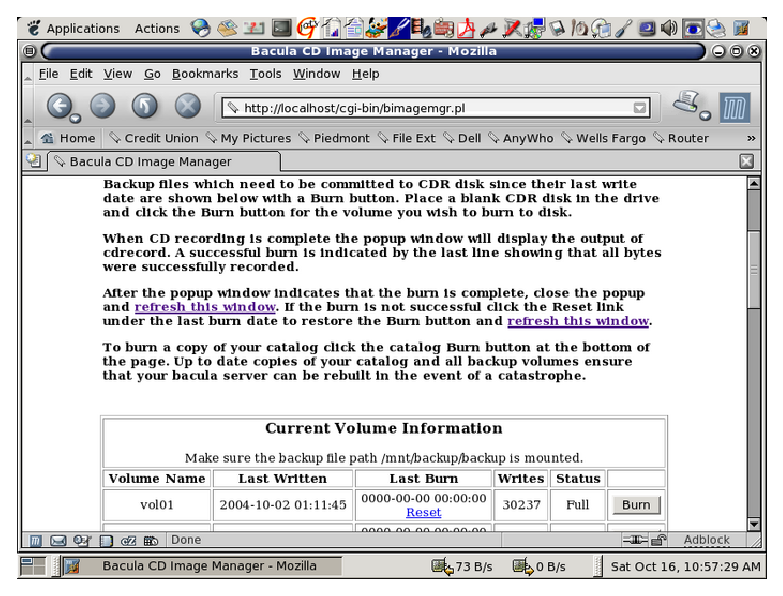
\includegraphics{./bimagemgr1.eps} \\Figure 1 

Place a blank CDR disk in your recorder and click a ``Burn'' button. This will
cause a pop up window as shown in Figure 2 to display the burn progress. 

\addcontentsline{lof}{figure}{Bacula CD Image Burn Progress Window}
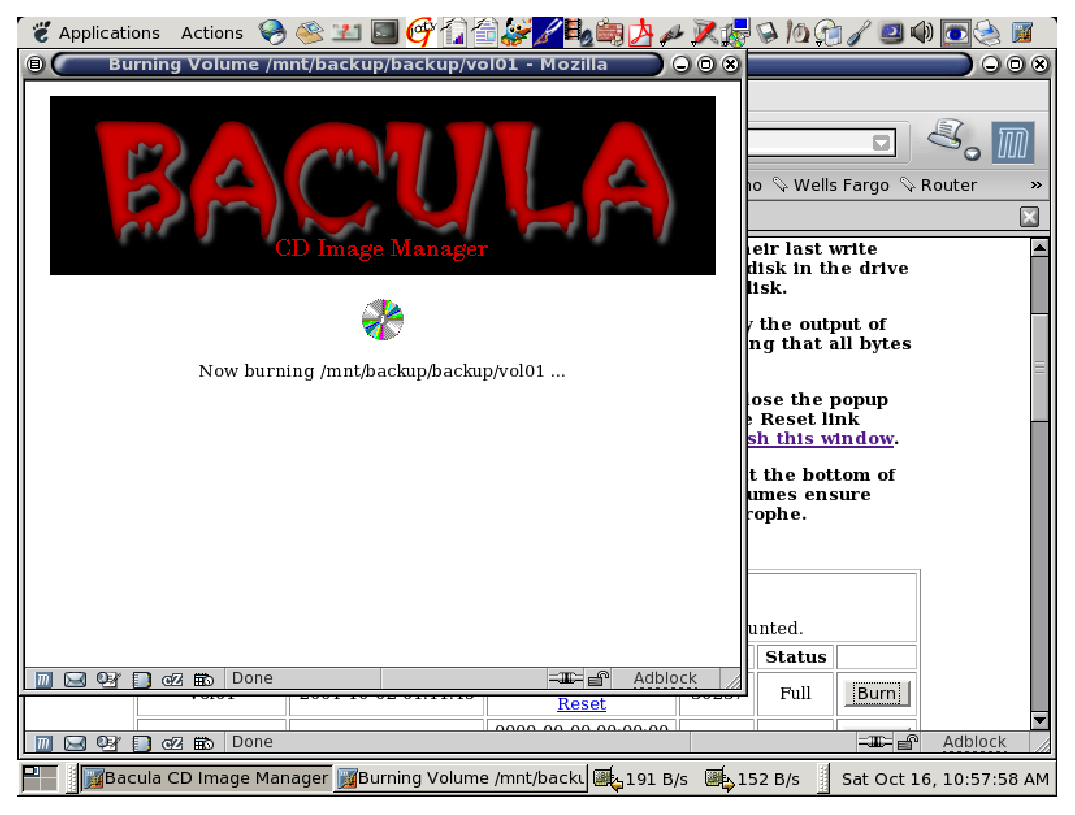
\includegraphics{./bimagemgr2.eps} \\Figure 2 

When the burn finishes the pop up window will display the results of cdrecord
as shown in Figure 3. Close the pop up window and refresh the main window. The
last burn date will be updated and the ``Burn'' button for that volume will
disappear. Should you have a failed burn you can reset the last burn date of
that volume by clicking it's ``Reset'' link. 

\addcontentsline{lof}{figure}{Bacula CD Image Burn Results}
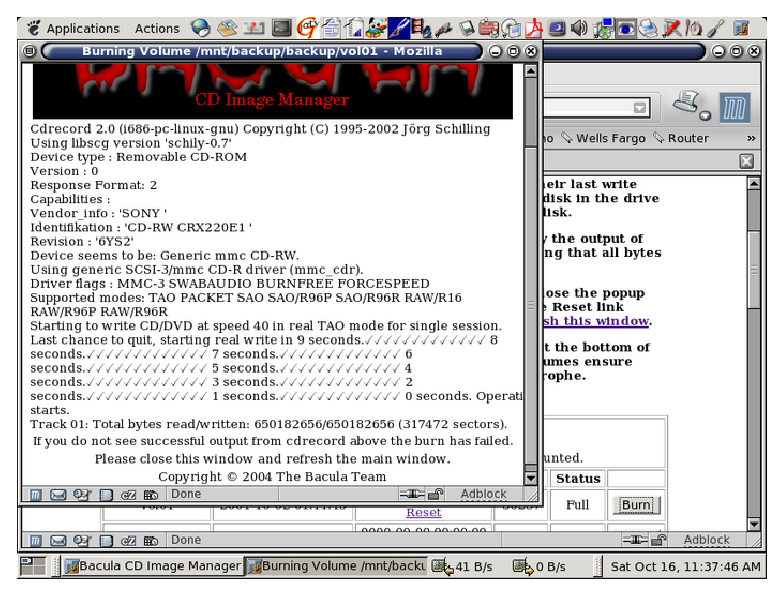
\includegraphics{./bimagemgr3.eps} \\Figure 3 

In the bottom row of the main display window are two more buttons labeled
``Burn Catalog'' and ``Blank CDRW''. ``Burn Catalog'' will place a copy of
your bacula catalog on a disk. If you use CDRW disks rather than CDR then
``Blank CDRW'' allows you to erase the disk before re-burning it. Regularly
committing your backup volume files and your catalog to disk with {\bf
bimagemgr} insures that you can rebuild easily in the event of some disaster
on the bacula server itself. 
